\section{Multidisciplinary Shape Sensitivity Analysis}
% =============================
The shape sensitivity analysis for the coupled multidisciplinary problem is built on the work done in Chapter \ref{ch:shapeSenwithIB}. However, in this chapter, we are also including the shape sensitivity effects on the structural side. To do so, we differentiate Equations \eqref{eq:C5_fluidGE} and \eqref{eq:C5_solidGE} alongside the kinematic and dynamic constraints of Equation \eqref{eq:C5_FSIconstraints} with respect to shape design variable, $b$. The sensitivity equations for the fluid and solid domains are shown in Equation \eqref{eq:C5_fluidSA} and \eqref{eq:C5_solidSA}, respectively.
%
\begin{subequations}\label{eq:C5_fluidSA}
\begin{align}
	&\rho^f \frac{\partial}{\partial t} \left( \frac{\partial \mathbf{u}^f}{\partial b} \right) + 
	\rho^f \frac{\partial \mathbf{u}^f}{\partial b} \cdot \nabla \mathbf{u}^f +
	\rho^f \mathbf{u}^f \cdot \nabla \left( \frac{\partial \mathbf{u}^f}{\partial b} \right) = 
	\nabla \cdot \left( \frac{\partial \mathbf{\sigma}^f}{\partial b} \right) +
	\rho^f \frac{\partial \mathbf{f}^f}{\partial b}
	\\
	&\nabla \cdot \left( \frac{\partial \mathbf{u}^f}{\partial b} \right) = 0
	\\
	&\frac{\partial \mathbf{\sigma}^f}{\partial b} = 
	\mu \left[ \nabla \left( \frac{\partial \mathbf{u}^f}{\partial b} \right) + 
	           \nabla \left( \frac{\partial \mathbf{u}^f}{\partial b} \right)^T \right] - 
	\frac{\partial p^f}{\partial b} \mathbf{I}
\end{align}
\end{subequations}
%
\begin{subequations}\label{eq:C5_solidSA}
\begin{align}
	\rho^s \frac{\partial \dot{\mathbf{u}}^s}{\partial b} &= 
	\nabla \cdot \left( \frac{\partial \sigma^s}{\partial b} \right) + 
	\frac{\partial \mathbf{f}^s}{\partial b}
	\\
	\frac{\partial \mathbf{\epsilon^s}}{\partial b} &=
	\frac{1}{2}
	\left[ \nabla \frac{\partial \mathbf{d}^s}{\partial b} + \nabla \left( \frac{\partial \mathbf{d}^s}{\partial b} \right)^T \right]
	\\
	\frac{\partial \mathbf{\sigma}^s}{\partial b} &= 
	\frac{\partial \mathbf{C}}{\partial b} : \mathbf{\epsilon}^s + 
	\mathbf{C} : \frac{\partial \mathbf{\epsilon}^s}{\partial b}
\end{align}
\end{subequations}
%
%
%\begin{subequations}\label{eq:C5_FSIconstraintsSA}
%\begin{align}
%	\frac{\partial \mathbf{u}^s}{\partial b} - 
%	\frac{\partial \mathbf{u}^f}{\partial b} &= 0
%	\\
%	\frac{\partial \mathbf{\sigma}^s}{\partial b} \cdot \mathbf{n} - 
%	\frac{\partial \mathbf{\sigma}^f}{\partial b} \cdot \mathbf{n} &= 0
%\end{align}
%\end{subequations}
\begin{subequations}\label{eq:C5_FSIconstraintsSA}
\begin{align}
	\frac{D \mathbf{u}^s}{D b} - 
	\frac{D \mathbf{u}^f}{D b} &= 0
	\\
	\frac{D \mathbf{\sigma}^s}{D b} \cdot \mathbf{n} - 
	\frac{D \mathbf{\sigma}^f}{D b} \cdot \mathbf{n} &= 0
\end{align}
\end{subequations}
%
The derivatives of the interface conditions of Equation \eqref{eq:C5_FSIconstraintsSA} are written and simplified using the chain rule. Here we show the process for the Dirichlet boundary condition. The same approach can be made for the Neumann boundaries as well.
%
\begin{gather*}
	\overbrace{	
	\left(
	\frac{\partial \mathbf{u}^s}{\partial b} +
	\frac{\partial \mathbf{u}^s}{\partial \mathbf{x}^s} \frac{\partial \mathbf{x}^s}{\partial b} +
	\frac{\partial \mathbf{u}^s}{\partial \mathbf{x}^f} \frac{\partial \mathbf{x}^f}{\partial b}
	\right)
	}^{\dfrac{D \mathbf{u}^s}{D b}} -
	\overbrace{
	\left(
	\frac{\partial \mathbf{u}^f}{\partial b} +
	\frac{\partial \mathbf{u}^f}{\partial \mathbf{x}^s} \frac{\partial \mathbf{x}^s}{\partial b} +
	\frac{\partial \mathbf{u}^f}{\partial \mathbf{x}^f} \frac{\partial \mathbf{x}^f}{\partial b}
	\right)
	}^{\dfrac{D \mathbf{u}^f}{D b}} = 0 \Longrightarrow
	\\
	\left(
	\frac{\partial \mathbf{u}^s}{\partial b} - \frac{\partial \mathbf{u}^f}{\partial b}
	\right) +
	\left(
	\frac{\partial \mathbf{u}^s}{\partial \mathbf{x}^s} - 
	\frac{\partial \mathbf{u}^f}{\partial \mathbf{x}^s}
	\right) \frac{\partial \mathbf{x}^s}{\partial b} +
	\left(
	\frac{\partial \mathbf{u}^s}{\partial \mathbf{x}^f} - 
	\frac{\partial \mathbf{u}^f}{\partial \mathbf{x}^f}
	\right) \frac{\partial \mathbf{x}^f}{\partial b} = 
	0 \Longrightarrow
	\\
	\left(
	\frac{\partial \mathbf{u}^s}{\partial b} - \frac{\partial \mathbf{u}^f}{\partial b}
	\right) +
	\frac{\partial }{\partial \mathbf{x}^s}
	\underbrace{	
	\left(
	\mathbf{u}^s - \mathbf{u}^f
	\right)
	}_{=\mathbf{0}} \frac{\partial \mathbf{x}^s}{\partial b} +
	\frac{\partial }{\partial \mathbf{x}^f}
	\underbrace{	
	\left(
	\mathbf{u}^s - \mathbf{u}^f
	\right)
	}_{=\mathbf{0}} \frac{\partial \mathbf{x}^f}{\partial b} = 
	0 \Longrightarrow
	\\
	\frac{\partial \mathbf{u}^s}{\partial b} - 
	\frac{\partial \mathbf{u}^f}{\partial b} = 0
\end{gather*}
%
The sensitivity of solid shape movement is represented in the derivative of the forcing function, $\mathbf{f}^f$ in Equation \eqref{eq:C5_fluidSA}. In particular, the geometric sensitivity of the solid boundary is added to the governing equations through the derivative of the regularized delta function in Equation \eqref{eq:C5_fluidSA}. However, as discussed in Chapter \ref{ch:sensitivityAnalysis}, the geometric sensitivity does not propagate inside the domain since the fluid mesh does not move.

To solve the sensitivity equations we need to obtain the solution of the governing equation ($\mathbf{u}^f$, $\mathbf{\epsilon^s}$). Therefore, we are proposing to use the flowchart of Figure \ref{fig:C5_SAflowchart} for the coupled multidisciplinary sensitivity analysis. The sensitivity calculation process starts by solving the Navier-Stokes equation and mapping the pressure to the structural domain to calculate the deformation in the structural domain. The solution of the Navier-Stokes and Elasticity equations are then fed to the sensitivity solver to calculate the sensitivity response. This loop is continued until a convergence for the governing equations is reached, or the process is stopped manually. 
%
\begin{figure}[H]
    \centering
    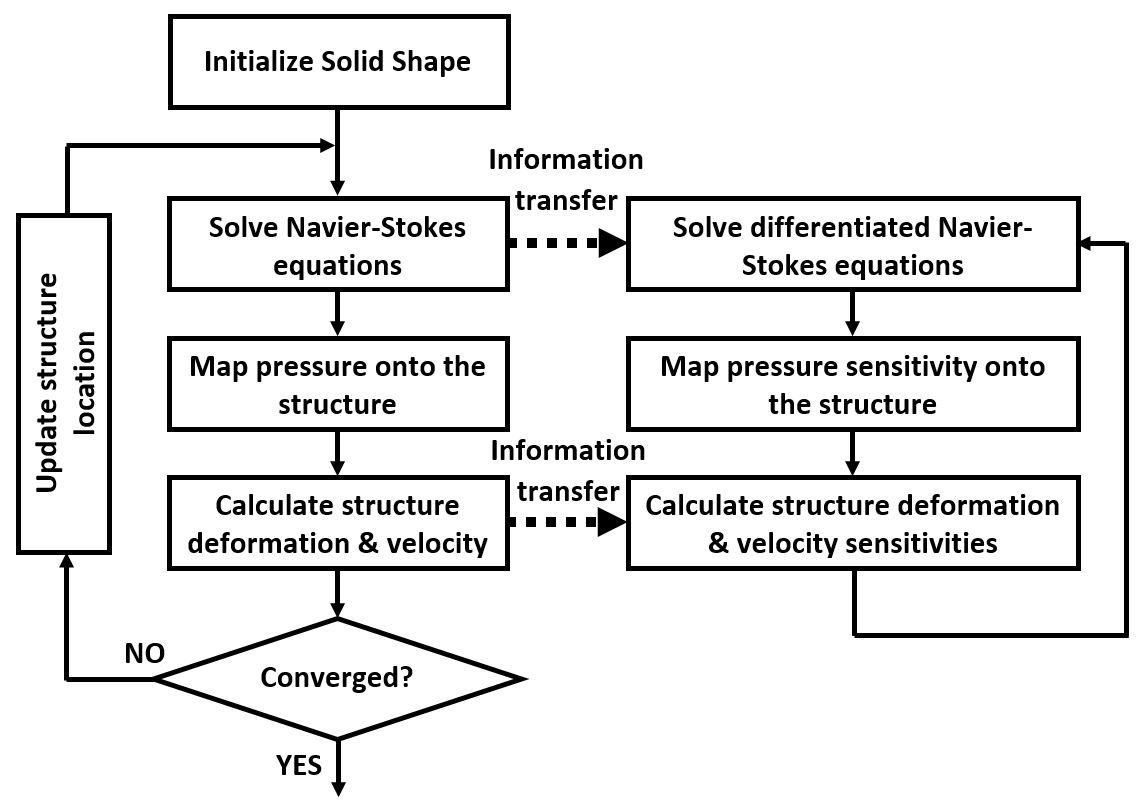
\includegraphics[width=14.00cm]{Chapter_5/figure/couple_SA_flowchart.jpg}
    \caption{Coupled multidisciplinary sensitivity analysis flowchart. The loop represents time marching for solution convergence.}
    \label{fig:C5_SAflowchart}
\end{figure}
%